\documentclass{llncs}
\usepackage{times}
\usepackage[T1]{fontenc}

% Comentar para not MAC Users
%\usepackage[applemac]{inputenc}

\usepackage{a4}
%\usepackage[margin=3cm,nohead]{geometry}
\usepackage{epstopdf}
\usepackage{indentfirst}
\usepackage{graphicx}
\usepackage{float}
\usepackage{fancyvrb}
\usepackage{amsmath}
\usepackage{color}
%\renewcommand{\baselinestretch}{1.5}

\begin{document}
\mainmatter
\title{TP2: Protocolo IP (Parte2)}

\titlerunning{TP2: Protocolo IP (Parte2)}

\author{Diogo Braga \and João Silva \and Ricardo Caçador}

\authorrunning{Diogo Braga \and João Silva \and Ricardo Caçador}

\institute{
University of Minho, Department of  Informatics, 4710-057 Braga, Portugal\\
e-mail: \{a82547,a82005,a81064\}@alunos.uminho.pt\\
PL4, Grupo 7
}

\date{}
\bibliographystyle{splncs}

\maketitle

\section{Endereçamento e Encaminhamento IP}
\emph{Considere que a organização MIEI-RC é constituída por três departamentos (A, B, e C) e cada departamento possui um router de acesso à sua rede local. Estes routers de acesso (Ra, Rb, e Rc) estão interligados entre si por ligações Ethernet a 1Gbps, formando um anel. Por sua vez, existe um servidor (S1) na rede do departamento C e, pelo menos, três laptops por departamento, interligados ao router respetivo através de um comutador (switch). S1 tem uma ligação a 1Gbps e os laptops ligações a 100Mbps. Considere apenas a existência de um comutador por departamento.}

\emph{A conectividade IP externa da organização é assegurada através de um router de acesso Rext conectado a Rc por uma ligação ponto-a-ponto a 10 Gbps.}

\emph{Construa  uma  topologia  CORE que reflita a rede local da  empresa. Para  facilitar  a visualização pode ocultar o endereçamento IPv6.}

\subsection{Exercício 1}
\emph{Atenda aos endereços IP atribuídos automaticamente pelo CORE aos diversos equipamentos da topologia.}

\subsubsection{a)}
\emph{Indique que endereços IP e máscaras de rede foram atribuídos pelo CORE a cada equipamento. Para simplificar, pode incluir uma imagem que ilustre de forma clara a topologia definida e o endereçamento usado.}
\\ \par
\textbf{R:} Na seguinte figura encontra-se a topologia de rede definida bem como todos os endereços IP atribuídos a cada equipamento da rede.

\begin{figure}[H]
\begin{center}
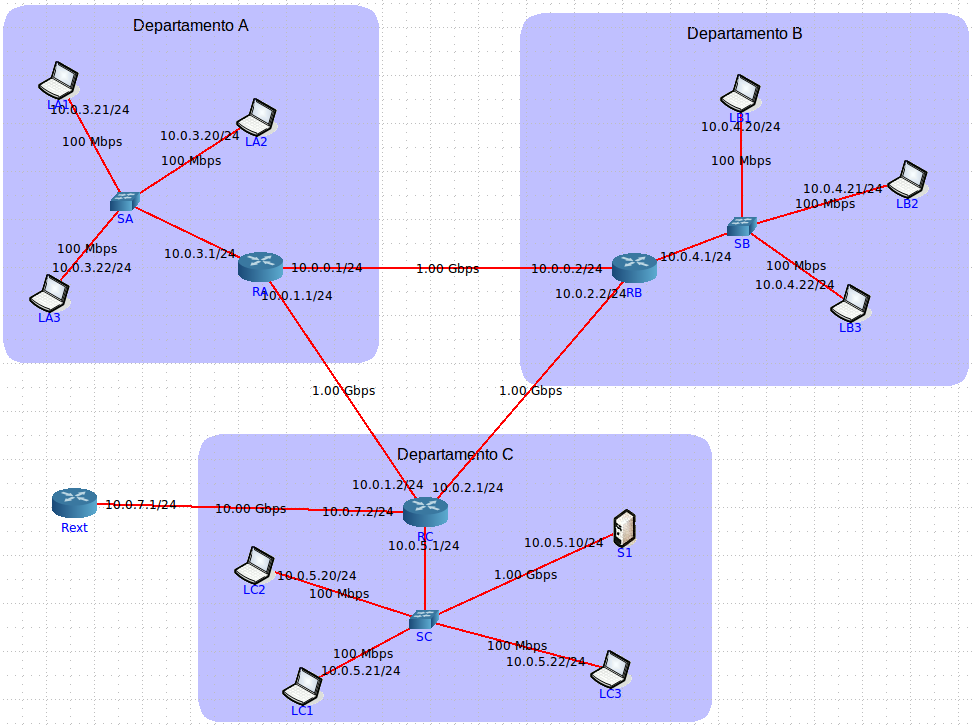
\includegraphics[scale=0.25]{1_a.png} 
\end{center}
\caption{\label{fig:1_a} Topologia definida.}
\end{figure} 

\subsubsection{b)}
\emph{Tratam
-
se de endereços públicos ou privados
?
Porquê?}
\\ \par
\textbf{R:} Segundo o \textbf{RFC1918}, a IANA (Internet Assigned Numbers Authority) reservou o espaço de endereçamento 10.0.0.0 - 10.255.255.255, para internets privadas. Como se pode observar na figura \ref{fig:1_a}, todos os equipamentos estão endereçados dentro deste espaço, conclui-se então que os endereços são \textbf{privados}.

\subsubsection{c)}
\emph{Porque razão não é atribuído um endereço IP aos 
switches?}
\\ \par
\textbf{R:} Um endereço IP é um requisito para a camada de rede (nível 3), os switches trabalham estritamente na camada link (nível 2) e, portanto, não precisam de um endereço IP.

\subsubsection{d)}
\emph{Usando o comando 
ping
certifique-se que existe conectividade 
IP
entre
os 
laptops
dos vários  departamentos e o servidor do  departamento  C (basta certificar-se da conectividade de um laptop por departamento).}
\\ \par
\textbf{R:} Usando o comando ping testamos a existência de conectividade entre departamentos, e dos departamentos com o servidor S1.

Existe conectividade entre o Departamento C e o Departamento A, podemos verificar isso na figura \ref{fig:lc1_la1} onde conectamos o os laptops LC1 e LA1 (10.0.3.21). O departamento C também tem conectividade com o servidor S1, como se pode verificar na figura \ref{fig:lc1_s1}.

\begin{figure}[H]
\begin{center}
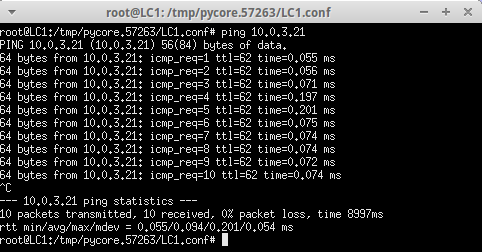
\includegraphics[scale=0.50]{LC1_LA1.png} 
\end{center}
\caption{\label{fig:lc1_la1} Conexão entre departamento C e departamento A.}
\end{figure} 

\begin{figure}[H]
\begin{center}
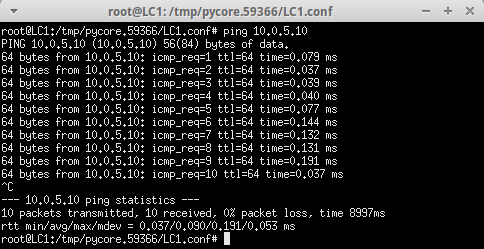
\includegraphics[scale=0.50]{LC1_S1.png} 
\end{center}
\caption{\label{fig:lc1_s1} Conexão entre departamento C e o servidor S1.}
\end{figure} 


Existe conectividade entre o Departamento C e o Departamento B, podemos verificar isso na figura \ref{fig:lc1_lb1} onde conectamos o os laptops LC1 e LB1 (10.0.4.20).

\begin{figure}[H]
\begin{center}
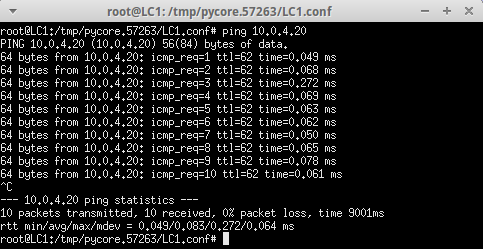
\includegraphics[scale=0.50]{LC1_LB1.png} 
\end{center}
\caption{\label{fig:lc1_lb1} Conexão entre departamento C e o departamento B.}
\end{figure} 

Existe conectividade entre o Departamento A e o Departamento B, podemos verificar isso na figura \ref{fig:la1_lb1} onde conectamos o os laptops LA1 e LB1 (10.0.4.20). O departamento A também tem conectividade com o servidor S1, como se pode verificar na figura \ref{fig:la1_s1}.

\begin{figure}[H]
\begin{center}
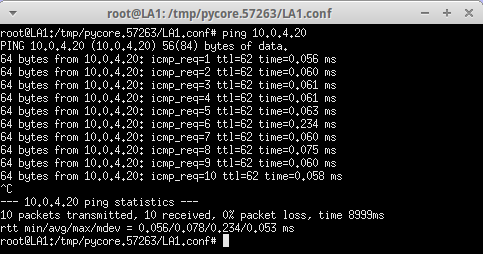
\includegraphics[scale=0.50]{LA1_LB1.png} 
\end{center}
\caption{\label{fig:la1_lb1} Conexão entre departamento A e o departamento B.}
\end{figure} 

\begin{figure}[H]
\begin{center}
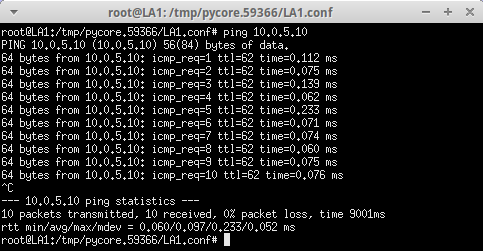
\includegraphics[scale=0.50]{LA1_S1.png} 
\end{center}
\caption{\label{fig:la1_s1} Conexão entre departamento A e o servidor S1.}
\end{figure} 

O departamento B tem conectividade com o servidor S1, como se pode verificar na figura \ref{fig:lb1_s1}.

\begin{figure}[H]
\begin{center}
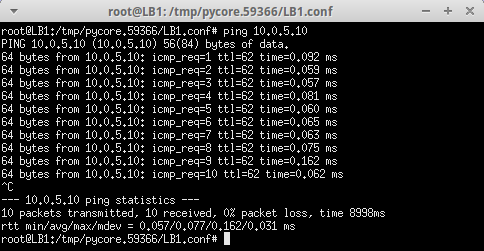
\includegraphics[scale=0.50]{LB1_S1.png} 
\end{center}
\caption{\label{fig:lb1_s1} Conexão entre departamento B e o servidor S1.}
\end{figure} 

\subsubsection{e)}
\emph{Verifique  se  existe  conectividade IP do router de acesso Rext para o servidor S1.}
\\ \par
\textbf{R:} Existe conetividade entre o servidor S1 e o router externo Rext, como se pode ver na figura \ref{fig:rext_s1}, onde se testa a conetividade do router de acesso para o servidor.

\begin{figure}[H]
\begin{center}
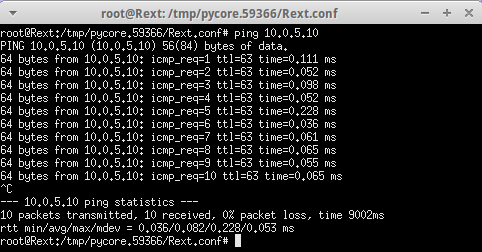
\includegraphics[scale=0.50]{REXT_S1.png} 
\end{center}
\caption{\label{fig:rext_s1} Conexão entre router de acesso Rext e o servidor S1.}
\end{figure} 

\subsection{Exercício 2}
\emph{Para o router e um laptop do departamento A:}

\subsubsection{a)}
\emph{Execute o comando netstat –rn por forma a poder consultar a tabela de encaminhamento unicast (IPv4). Inclua no seu relatório as tabelas de encaminhamento obtidas; interprete as várias entradas de cada tabela. Se necessário, consulte o manual respetivo (man netstat). }
\\ \par
\textbf{R:} Pode-se ver na figura \ref{fig:netstat_la1} a tabela de encaminhamento do laptop LA1, e na figura \ref{fig:netstat_ra} a tabela de encaminhamento do router RA.

\begin{figure}[H]
\begin{center}
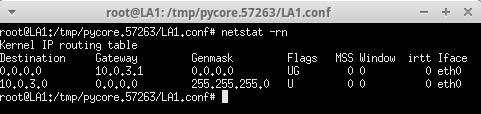
\includegraphics[scale=0.50]{netstat_LA1.png} 
\end{center}
\caption{\label{fig:netstat_la1} Tabela de encaminhamento do laptop LA1.}
\end{figure} 

\begin{figure}[H]
\begin{center}
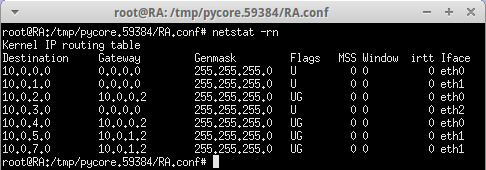
\includegraphics[scale=0.60]{netstat_RA.png} 
\end{center}
\caption{\label{fig:netstat_ra} Tabela de encaminhamento do router RA.}
\end{figure} 

Na tabela de encaminhamento do laptop LA1, os únicos endereços de saída são o respetivo router do departamento por onde saem todos os packets destinados a outros departamentos ou outras redes, e no caso de querer comunicar com laptops no próprio departamento, os datagramas serão entregues na interface de endereço próprio que corresponde ao gateway 0.0.0.0, sendo isto feito com auxílio do Ethernet Switch.

Na tabela de encaminhamento do router do departamento A, dependendo para onde se quer enviar os datagramas usamos endereços de saída diferentes. No caso de se querer enviar datagramas para o departamento B (10.0.4.0) usa-se interface de endereço 10.0.0.2. No caso de se querer enviar datagramas para o departamento C (10.0.5.0) usa-se interface de endereço 10.0.1.2. No caso de se querer comunicar com as redes adjacentes usa-se a interface de endereço default (0.0.0.0). Por último, no caso de se querer comunicar com redes exteriores à topologia criada para os departamentos (10.0.7.0) usa-se a interface de endereço 10.0.1.2. 

\subsubsection{b)}
\emph{Diga,  justificando, se  está  a  ser  usado  encaminhamento  estático  ou dinâmico (sugestão: analise  que  processos  estão  a  correrem cada sistema).}
\\ \par
\textbf{R:} Este sistema possui encaminhamento dinâmico e estático. Na topologia de rede em anel (Router A - Router B - Router C) o encaminhamento é dinâmico. Desta forma, as rotas são atualizadas ao longo do tempo e, caso exista alguma falha num link entre routers, existe adaptação a um novo caminho.

Em cada departamento, o encaminhamento entre os equipamentos é realizado de forma estática. Este tipo de encaminhamento é baseado em rotas pré-definidas, visto estarmos perante topologias de rede em que existe maior conhecimento entre os intervenientes. O mesmo acontece na ligação entre o Router C e o Router RExt.

\begin{figure}[H]
\begin{center}
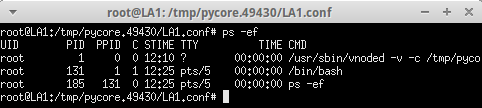
\includegraphics[scale=0.60]{2b1.png} 
\end{center}
\caption{\label{fig:2b1} Processos a decorrer no laptop LA1.}
\end{figure}

\begin{figure}[H]
\begin{center}
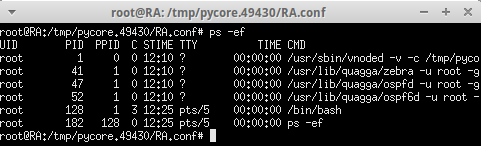
\includegraphics[scale=0.60]{2b2.png} 
\end{center}
\caption{\label{fig:2b2} Processos a decorrer no router RA.}
\end{figure}

Podemos verificar na imagem \ref{fig:2b1} que apenas temos 3 processos a decorrer na
máquina: o processo-pai, a bash e o comando ps.

Podemos verificar na imagem \ref{fig:2b2} que temos 6 processos a decorrer na
máquina: o processo-pai, a bash, o comando ps e 3 deamons, 2 dois quais são protocolos
de roteamento para IPv4 e IPv6.

Desta forma, concluimos que nos routers existe encaminhamento dinâmico, e nos laptops
encaminhamento estático.

\subsubsection{c)}
\emph{Admita que, por questões administrativas, a rota por defeito (0.0.0.0 ou default) deve ser retirada definitivamente da tabela de encaminhamento do servidor S1 localizado  no departamento C. Use o comando route delete para o efeito. Que  implicações  tem  esta  medida  para  os utilizadores da empresa que acedem ao servidor. Justifique.}
\\ \par
\textbf{R:} Pode-se ver na figura \ref{fig:2c} a aplicação do comando \emph{route delete} no servidor S1, assim como a tabela de encaminhamento antes e depois do sucedido, que comprova o sucesso do comando realizado.

\begin{figure}[H]
\begin{center}
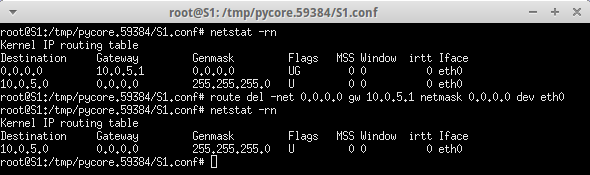
\includegraphics[scale=0.60]{2c.png} 
\end{center}
\caption{\label{fig:2c} Utilização do comando route delete.}
\end{figure}

Ao retirar a rota por defeito da tabela de encaminhamento do servidor S1, os utilizadores da empresa que por norma acedem ao servidor deixam de poder fazer tal acesso, pois foi retirado o endereço de saída 10.0.5.1 com que o servidor se ligava ao switch que por sua vez se ligava ao Router C. 

Sempre que os utilizadores tentam comunicar com o servidor S1, enviam os seus packets mas não recebem resposta do servidor uma vez que este já não tem como comunicar com o exterior do departamento C, logo a rota não é definida e a comunicação não é estabelecida.

Um exemplo disso é o teste de conexão do laptop LA1 ao servidor S1, como se pode ver na figura \ref{fig:2c_2}.

O servidor apenas consegue conectar com laptops dentro do departamento C uma vez que estes tem o endereço que combina com 10.0.5.0, essa conexão pode ser vista na figura \ref{fig:2c_3}.

\begin{figure}[H]
\begin{center}
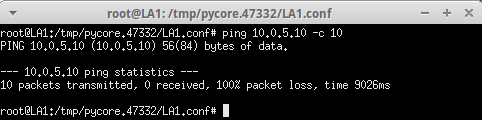
\includegraphics[scale=0.60]{2c_2.png} 
\end{center}
\caption{\label{fig:2c_2} Teste de conexão entre LA1 e o S1.}
\end{figure}

\begin{figure}[H]
\begin{center}
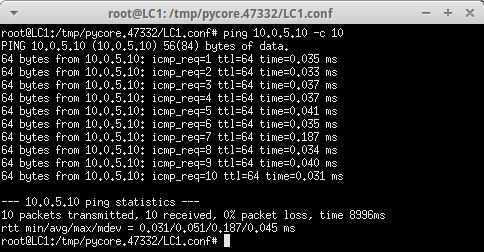
\includegraphics[scale=0.60]{2c_3.png} 
\end{center}
\caption{\label{fig:2c_3} Teste de conexão entre LC1 e o S1.}
\end{figure}

\subsubsection{d)}
\emph{Adicione as rotas estáticas necessárias para restaurar a conectividade para o servidor S1, por forma a contornar a restrição imposta na alínea c). Utilize para o efeito o comando route add e registe os comandos que usou.}
\\ \par
\textbf{R:} Pode-se ver na figura \ref{fig:2d} que a aplicação do comando Route Add no servidor S1, assim como a tabela de encaminhamento antes e depois do sucedido, que comprova o sucesso do comando realizado.

\begin{figure}[H]
\begin{center}
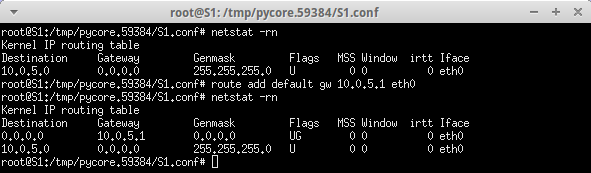
\includegraphics[scale=0.60]{2d.png} 
\end{center}
\caption{\label{fig:2d} Utilização do comando route add.}
\end{figure}

\subsubsection{e)}
\emph{Teste a nova política de encaminhamento garantindo que o servidor está novamente acessível, utilizando para o efeito o comando ping. Registe a nova tabela de encaminhamento do servidor.}
\\ \par
\textbf{R:} Pode se ver na figura \ref{fig:2e1} que a nova política de encaminhamento funciona corretamente e que o servidor está novamente acessível, através do teste de conectividade com o laptop de outro departamento, neste caso o laptop 1 do departamento B.
Pode-se ver na figura \ref{fig:2e2} a nova tabela de encaminhamento do servidor S1.

\begin{figure}[H]
\begin{center}
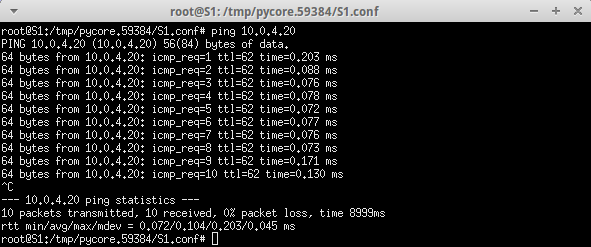
\includegraphics[scale=0.60]{2e1.png} 
\end{center}
\caption{\label{fig:2e1} Conexão entre o laptop LB1 e o servidor S1.}
\end{figure}

\begin{figure}[H]
\begin{center}
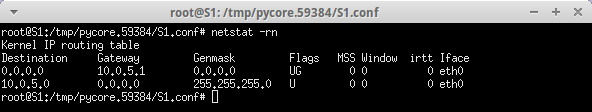
\includegraphics[scale=0.60]{2e2.png} 
\end{center}
\caption{\label{fig:2e2} Nova tabela de encaminhamento do servidor S1.}
\end{figure}

\section{Definição de Sub-redes}
\emph{Considere a topologia definida anteriormente. Assuma que o endereçamento entre os routers se mantém inalterado, contudo, o endereçamento em cada departamento deve ser redefinido. }

\subsection{1)}
\emph{Considere que dispõe apenas do endereço de rede IP 172.XX.48.0/20, em que XX é o decimal correspondendo ao seu número de grupo (PLXX). Defina um novo esquema de endereçamento para as redes dos departamentos (mantendo a rede de acesso e core inalteradas) e atribua endereços às interfaces dos vários sistemas envolvidos. Deve justificar as opções usadas.}
\\ \par
\textbf{R:} Pode se ver na figura \ref{fig:3_1} o novo de esquema de endereçamento para
as redes dos departamentos usando apenas o endereço de rede 172.47.48.0/20.

\begin{figure}[H]
\begin{center}
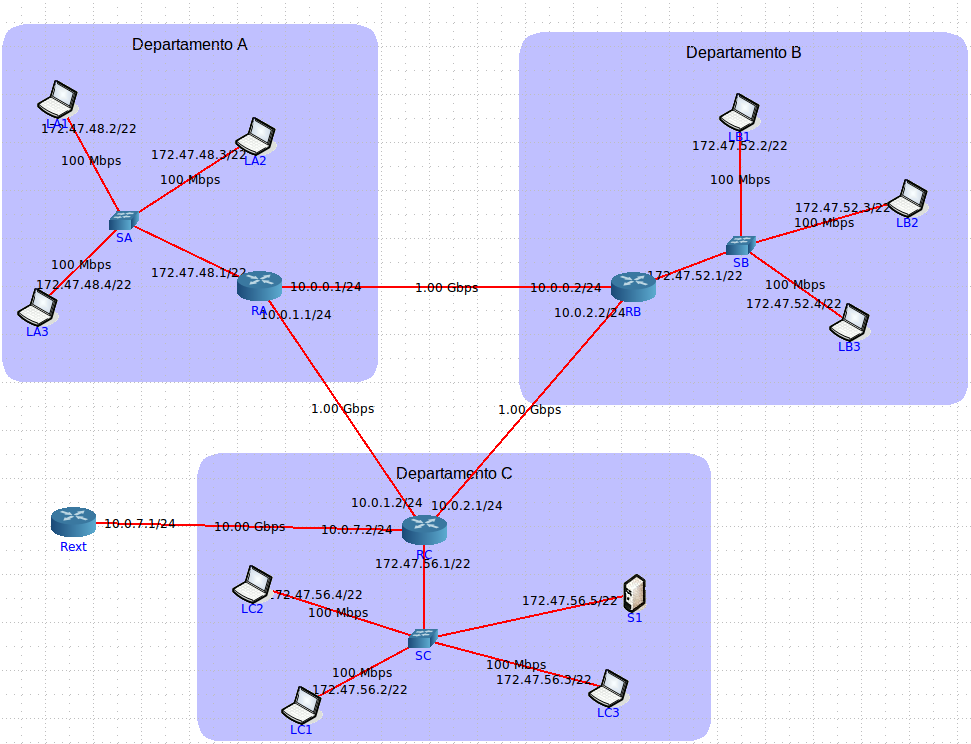
\includegraphics[scale=0.40]{3_1.png} 
\end{center}
\caption{\label{fig:3_1} Novo esquema de endereçamento.}
\end{figure}

O endereço 172.47.48.0/20 corresponde a 10101100.00101111.0011|0000.00000000. Os bits
antes da barra representam a rede, enquanto os bits posteriores representam os hosts.

Como necessitavamos de definir 3 subredes basta apenas alocar 2 bits para tal, ficando
assim a máscara de rede igual a /22. Desta forma conseguimos definir 4 novas subredes.

Para o departamento A, usamos a subrede 00, pelo que os hots são endereçados entre o
endereço 172.47.48.1/22 e o endereço 172.47.51.254/22.

Para o departamento B, usamos a subrede 01, pelo que os hots são endereçados entre o
endereço 172.47.52.1/22 e o endereço 172.47.55.254/22.

Para o departamento C, usamos a subrede 10, pelo que os hots são endereçados entre o
endereço 172.47.56.1/22 e o endereço 172.47.59.254/22.

\subsection{2)}
\emph{Qual a máscara de rede que usou (em formato decimal)? Quantos hosts IP pode interligar em cada departamento? Justifique.}
\\ \par
\textbf{R:} A máscara de rede usada foi /22. Como o endereço na totalidade possui 32 bits, e visto que os bits de identificação de rede são 20 e os de identificação de subrede são 2, ficam a sobrar 10 bits para endereçamento de hosts. Portanto, é possível em cada departamento endereçar ((2 elevado a 10)-2=) 1022 hosts. Os 2 endereços retirados estão reservados para broadcast e identificador de subrede.

Usamos 2 bits para definição de subredes pois é o menor número possível para criação
de 3 subredes.

\subsection{3)}
\emph{Garanta e verifique que conectividade IP entre as várias redes locais da organização MIEI-RC é mantida. Explique como procedeu.}
\\ \par
\textbf{R:} Pode se verificar nas figuras \ref{fig:3_LA1_LB1}, \ref{fig:3_LB1_LC1} e
\ref{fig:3_LC1_LA1} que a conectividade entre os departamentos da organização é
mantida.

\begin{figure}[H]
\begin{center}
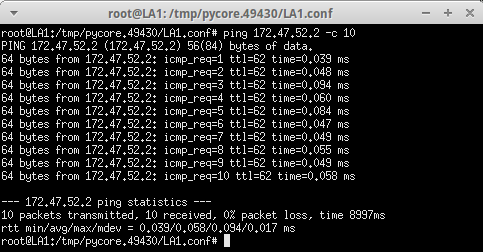
\includegraphics[scale=0.60]{3_LA1_LB1.png} 
\end{center}
\caption{\label{fig:3_LA1_LB1} Conectividade entre o equipamento LA1 e o LB1.}
\end{figure}

\begin{figure}[H]
\begin{center}
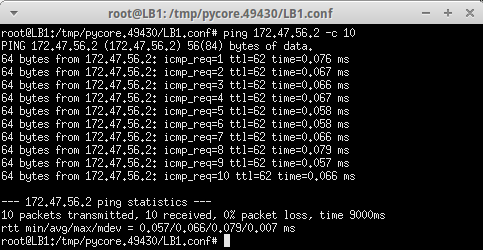
\includegraphics[scale=0.60]{3_LB1_LC1.png} 
\end{center}
\caption{\label{fig:3_LB1_LC1} Conectividade entre o equipamento LB1 e o LC1.}
\end{figure}

\begin{figure}[H]
\begin{center}
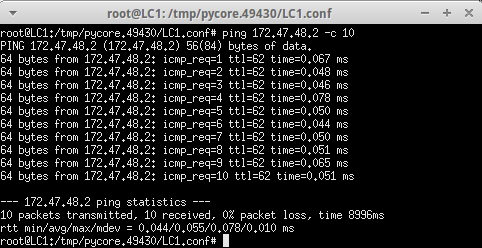
\includegraphics[scale=0.60]{3_LC1_LA1.png} 
\end{center}
\caption{\label{fig:3_LC1_LA1} Conectividade entre o equipamento LC1 e o LA1.}
\end{figure}

\section{Conclusões}



% exemplo de imagem
%\begin{figure}
%\begin{center}
%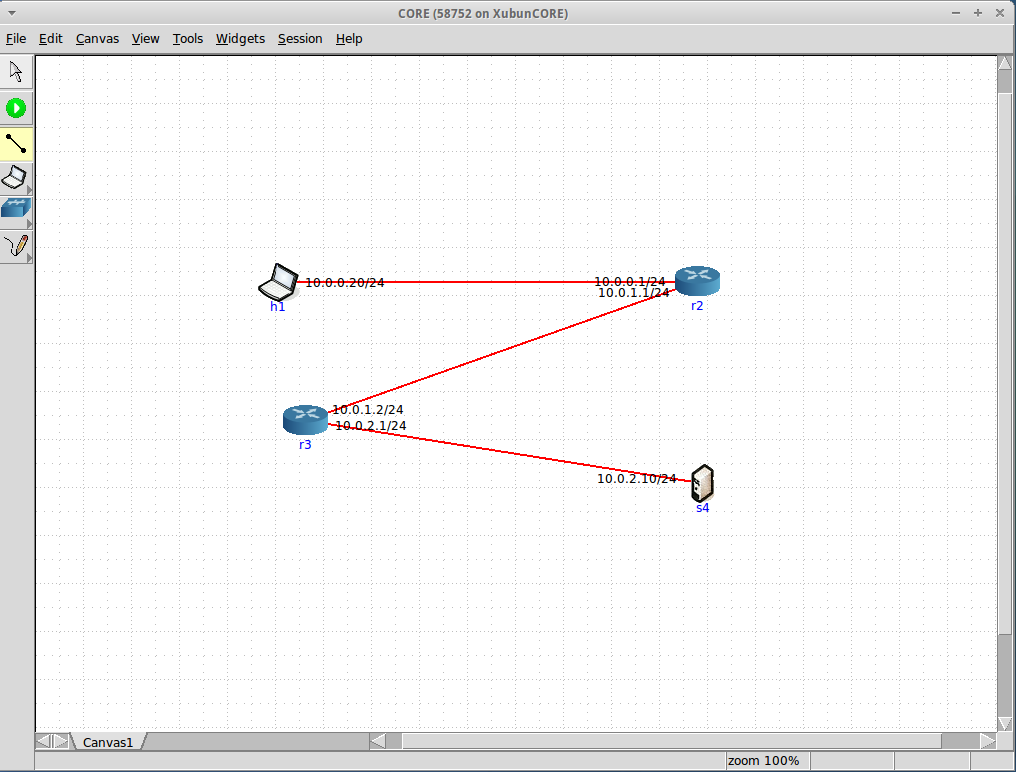
\includegraphics[scale=0.30]{intro.png} 
%\end{center}
%\caption{\label{fig:intro}Rede do exercício 1 do enunciado.}
%\end{figure} 




\end{document}